\section{Evaluation}  \label{sec:evaluation} 
The proposed obstacle aware controller\footnote{Source coude: \url{https://github.com/hubernikus/obstacle_aware_damping}} is compared to a baseline, the dyanmics preserving controller \cite{kronander2015passive}.


\subsection{Qualitative Comparison} \label{sec:qual_comp}
We first qualitatively observe the behavior of the proposed controller in different scenarios (Fig.~\ref{fig:obstacle_aware_damping_comparison}). The scenario entails three obstacles, which the agent is approaching from different starting positions. The time step is $0.01 s$, the agent has a mass matrix of $\matd{M} = \matr{I}$, and follwing damping values: 
$s^{\mathrm{obs}}=$\qty{200}{s^{-1}},
$s^{\mathrm{DS}}=$\qty{100}{s^{-1]}}, and
$s^{\mathrm{c}}=$\qty{20}{s^{-1}}.
In each scenario, a disturbance (arrow) is applied at the same time step.
The undisturbed trajectory is displayed for comparison.
% Based on this simulation, we can observe the robots' behavior in different scenarios.

The top trajectory, the robot is pushed towards the stand-alone obstacle. The obstacle aware controller safely avoids collision and continues to towards the attractor. Conversely, the baseline controller which focuses on conserving the dynamics is begin pushed into the obstacle. 
% a direction perpendicular to the desired motion. Since we want compliance in this direction and the robot is far from any obstacle, it deviates greatly from its previous trajectory. It continues its path to the attractor on another DS line.

In the middle trajectory, the disturbance happens when the agent is between two obstacles. We expect that the normal $\vect n(\vecs \xi)$ as used in the controller (Sec.~\ref{sec:obstacle_repulsion}.
However, by construction its magnitude becomes smaller in narrow passages, see \eqref{eq:averaged_normal}, and hence the damping increases, as described in \eqref{}.
As a result, the agent safely avoids the disturbance using the obstacle aware conroller. Whereas, the base line controller results in a colliding trajectory.

Finally, during the bottom trajectory, the repulsive force points away from the obstacle. Due to the compliance when moving away from and obstacle as define in \eqref{eq:leaving_compliance}, the obstacle aware and the dynamics preserving controller follow almost identical trajectories.
k
% Another disturbance (B) pushed the robot toward the obstacle and was successfully damped, avoiding the collision.

% A disturbance (C) pushed the robot away from an obstacle. The control algorithm is made such that when moving away from an obstacle, disturbances are not damped, and the robot shows compliant behavior. 

% The last disturbance (D) was applied along the direction of motion. As the desired behavior is damped in this direction, the robot almost kept the same speed and continued toward the attractor.

% \begin{figure}
% \centerline{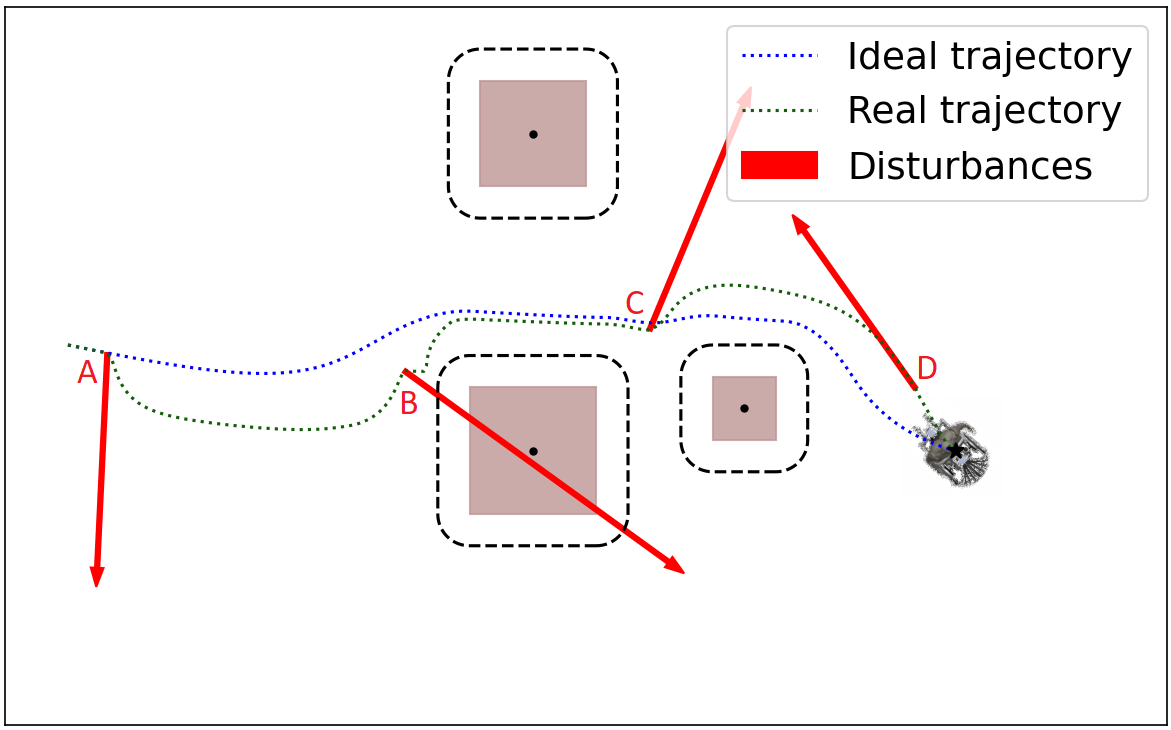
\includegraphics[width=0.5\textwidth]{figures/run_with_obs.png}}
% \caption{Simulation with a complex environment and disturbances applied to the robot}
% \label{fig_run_with_obs}
% \end{figure}

Furthermore, in Fig.~\ref{fig_run_damped_towards}, one can observe the feature described in Section~\ref{sec:damping_only_toward}, that only damps the disturbance towards the obstacle.
The first disturbance is highly damped, while the second is much less. This feature provides a natural behavior of moving away from obstacles, improving the margin of impenetrability. 

% The control law presented was tested in simulation in Python. The state space is the Cartesian coordinates $xy$ in 2D and $xyz$ in 3D. In practice, the damping matrix $\matd D(\vecs\xi)$ and the control command $\vecs {\tau_c}$ are recomputed at each time step.\\

% Let us compare traditional passive interaction control and the presented method (Fig.~\ref{fig_diff_obs_pass}). On the setup, the same disturbance is applied to both systems simultaneously. One can already see the robot equipped with traditional passive control (left) penetrates the obstacle, while ours (right) successfully damps the disturbance.

% \begin{figure}
% \centering
% \begin{subfigure}{0.8\columnwidth}
%   \centerline{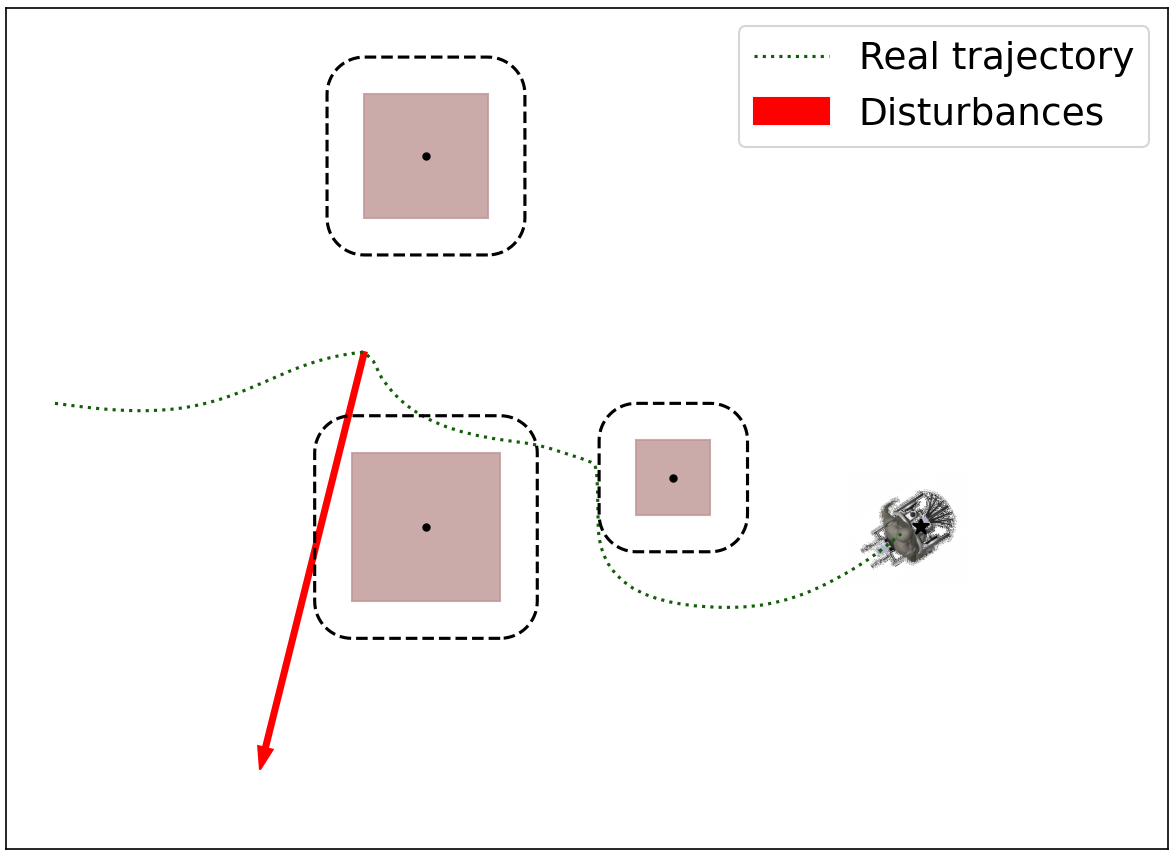
\includegraphics[width=\textwidth]{figures/run_without_pass.png}}
%   \caption{Traditional passive control}
% \end{subfigure}
% \begin{subfigure}{0.8\columnwidth}
%   \centerline{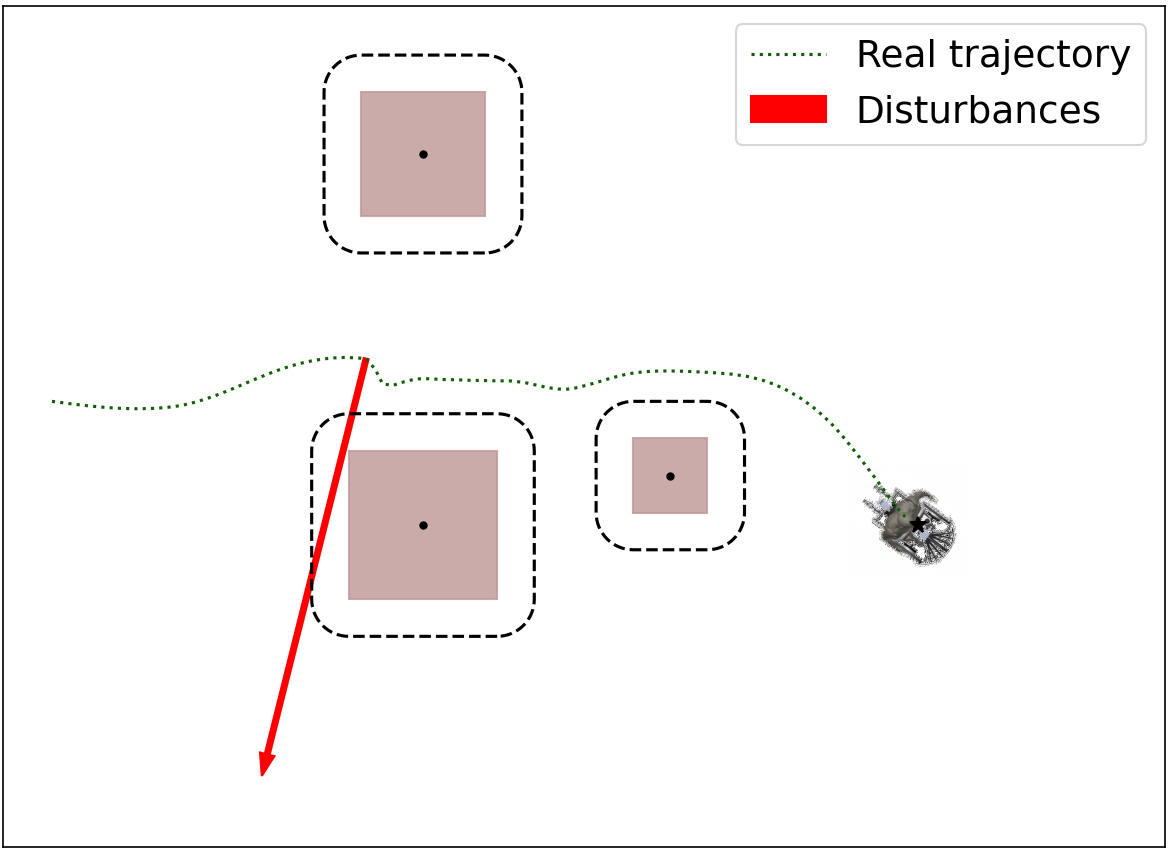
\includegraphics[width=\textwidth]{figures/run_with_pass.png}}
%   \caption{Obstacle aware passive control}
% \end{subfigure}
% \caption{Comparison of the two control methods}
% \label{fig:diff_obs_pass}
% \end{figure}

\begin{figure}
  \centering
  \centerline{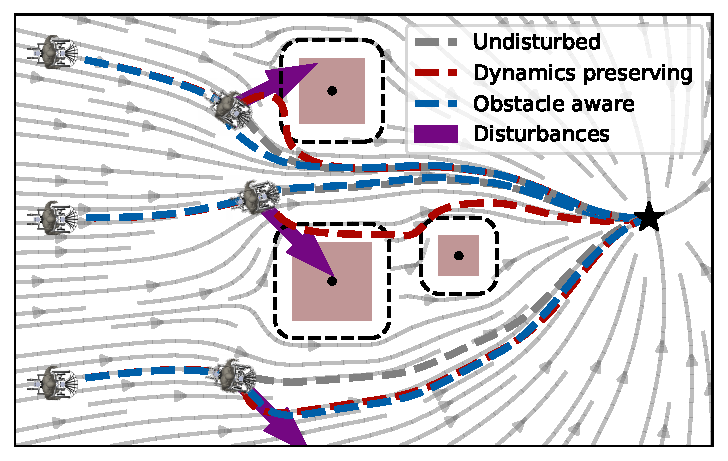
\includegraphics[width=0.95\columnwidth]{figures/multi_obstacle_with_damping.pdf}}
  % \centerline{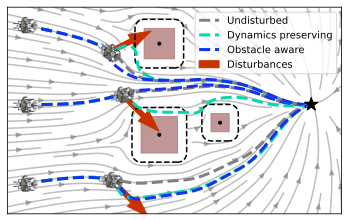
\includegraphics[width=0.5\textwidth]{figures/multi_obstacle_with_damping.svg}}
  \caption{The desired dynamics $\dot{\vecs \xi}$ in gray are as input for the force controller. 
  The mobile robot starting from the three positions, navigates safely to the attractor (black star) despite the disturbances (red arrows) when using the obstacle-aware controller.
  Conversely, the baseline (blue) leads to collision when the disturbance happens close to the robot.}
  \label{fig:obstacle_aware_damping_comparison}
\end{figure}

\subsection{Noise Analysis}
A real controller is always subject to noise, unexpected disturbances. This can be noise or inaccuracies in sensor readings, or small physical disturbances such as air drag for a fast moving drone, or floor roughness for a mobile robot. 
A high quality controller is able to reject such disturbances, while maintainingthe control ojbectives: collision avoidance and trajecotry tracking. 

This section looks at noise disturbance of a simulated agent with an identity mass matrix $\matd M = \matr I$. The discrete time step is chosen as $\Delta t = $\qty{0.2}{s}, furthermore the damping values are set as
$s^{\mathrm{obs}}=$\qty{50}{s^{-1}},
$s^{\mathrm{DS}}=$\qty{40}{s^{-1]}}, and
$s^{\mathrm{c}}=$\qty{5}{s^{-1}}.
% lambda_DS: 40.00
% lambda_perp: 5.00
% lambda_obs: 50.00
 The robot is tasked to follow a linear dynamics of  the form $\vect f(\vecs \xi) = (\vecs \xi^a -  \vecs \xi)$,nd the velocity is capped at a magnitude of \qty{1}{m/s}. 
 The controlless are compared by anaylyzing the minimal distance to the surface along a trajectory $ \min_t \| \vecs \xi_t - \vecs \xi^b \| $, see \eqref{eq:distance_function}.


\subsubsection{Velocity Noise Resistance}
In the first evaluation, normally distributed noise with mean of zero is added to the velocity $\dot{\vecs{ \xi}}$ before calulating the control force (Fig.~\ref{fig:velocity_noise}). Different variances of the noise are evaluated ranging from \qty{0}{m/s} to \qty{1.0}{m/s}. The start position is at $\vecs \xi_0 = [-2.5, 1.0]^T$ with an initial velocity of zero, and  the attractor at $\vecs \xi^a = [2.5, -1.0]^T$.
% The experiment is done on a simple setup with one obstacle. The noise added has a mean of $0$, and the standard deviation is increasing linearly from $0.0$ to $0.7m$ for position and $0.0$ to $7.0 \frac{m}{s}$ for velocity measurements. For each noise level, the simulation was run 10 times. The output variable is the smallest distance of the agent from the obstacle during the simulation. This metric was chosen to observe how the noise could lead to a crash in the obstacle. 

The obstacle aware controller is able to reject the noise acting on the velocity even with increasing noise variance. Nevertheless, the closest distance during the trajectory is decreasing with higerh values.
Conversely, the dynamics following has a mean distance which is below zero already at velocity noise variance of $\qty{0.5}{m/s}$, indicating a large number of trajectories colliding with at least one obstacle. 
It can futher be observed, without noise, the minimal distance along a trjaectory is higher for the obstacle aware controller. This is the result, that there is higher damping towards the obstacle, and hence the curvature of the dynamics guiding around the obstacle is followed more accurately.

\begin{figure}
    \centering
    \begin{subfigure}{\columnwidth}
      \centerline{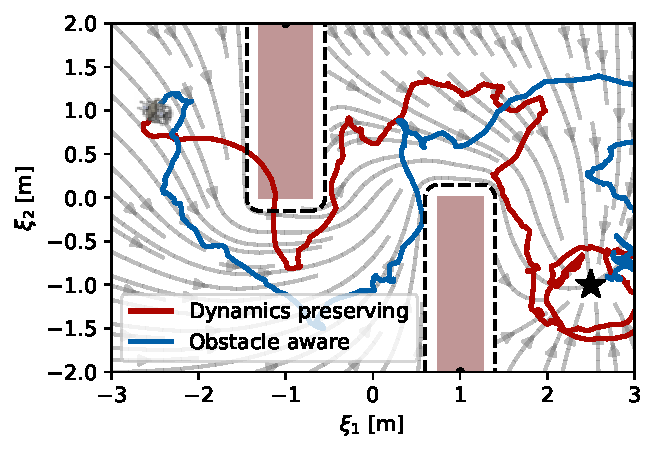
\includegraphics[width=\textwidth]{figures/trajectory_velocity_noise}}
      \caption{Trajectories with a standard deviation of the velocity-noise of 1.0 m/s.}
      \label{fig:trajectory_velocity_noise}
    \end{subfigure}
    \begin{subfigure}{\columnwidth}
    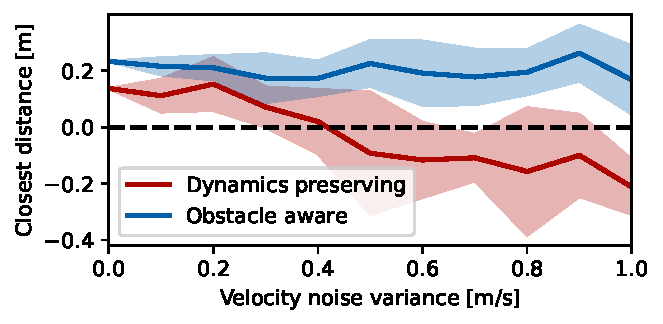
\includegraphics[width=\textwidth]{figures/comparison_velocity_noise}
      \caption{The mean and variance (shaded) of the closest distances over 10 epochs.}
      \label{fig:comparison_velocity_noise}
    \end{subfigure}
	\caption{An agent is navigating towards the attractor (black star) between two elongated obstacles (a), while white noise acting on the agent's velocity. The velocity noise has a mean of zero, and different variances between \qty{0.0}{m / s} and \qty{1.0}{m / s} are evaluated.}
\label{fig:velocity_noise}
\end{figure}

\subsubsection{Position Noise Resistance} \label{sec:position_noise}
In the second experiment, normally distributed noise with mean of zero is added to the position $\vecs{ \xi}$ (Fig.~\ref{fig:position_noise}). The variances of the noise are ranging from \qty{0.0}{m/s} to \qty{0.3}{m/s}. The start position is at $\vecs \xi_0 = [-2.5, -1.0]^T$ with an initial velocity of zero, and  the attractor at $\vecs \xi^a = [2.5, 1.0]^T$.
% For the noise acting on the position measurement, the controller presents good rejection for a small noise variance. As it increases, the robot's behavior quickly worsens (Fig.~\ref{fig_pos_noise}). The robot penetrates the obstacle for noises of standard deviation $ > 0.4 m$. An example of a run with $\sigma_{noise} = 0.7 m$ is shown in Fig.~\ref{fig_pos_noise_0_7}.

% The obstacle was never penetrated for the velocity measurement noise, asserting the robustness of the control for this type of noise (Fig.~\ref{fig_vel_noise}). Fig.~\ref{fig_2_vel_noise} provides an image of the simulation with big noise standard deviation ($4.0 \frac{m}{s}$). Thanks to the feature presented in Section~\ref{sec:damping_only_toward} (damping only toward the obstacle), the robot has even the tendency to drift away from the obstacle, increasing the safety margin.
Similarly to the previous evaluatoin, the obstacle aware controller maintains a greater distance to the surface with zero noise, where the dynamics preserving already collides.
This results in the means of the  distance above zero for standard deviations of the position noise smaller than \qty{0.023}{m} using the obstacle aware controller. Whereas, for the dynamics preserving controller, the mean of the distance to the surface is below zero, indicating collisions.
However, this is the result of the buffer that comes from the obstacle aware controller. 
As a similar decrease in distance is detected for both controllers. 

Furthermore, a higher variance of the distance is observed in the dynamics preserving controller. We assume that this comes from the fact, that the higher impedance of this controller makes it slower to adapt to a new velocity after being displaced by the noise. Hence, the velocity and the trajectory is more random. 

\begin{figure}
    \centering
    \begin{subfigure}{\columnwidth}
      \centerline{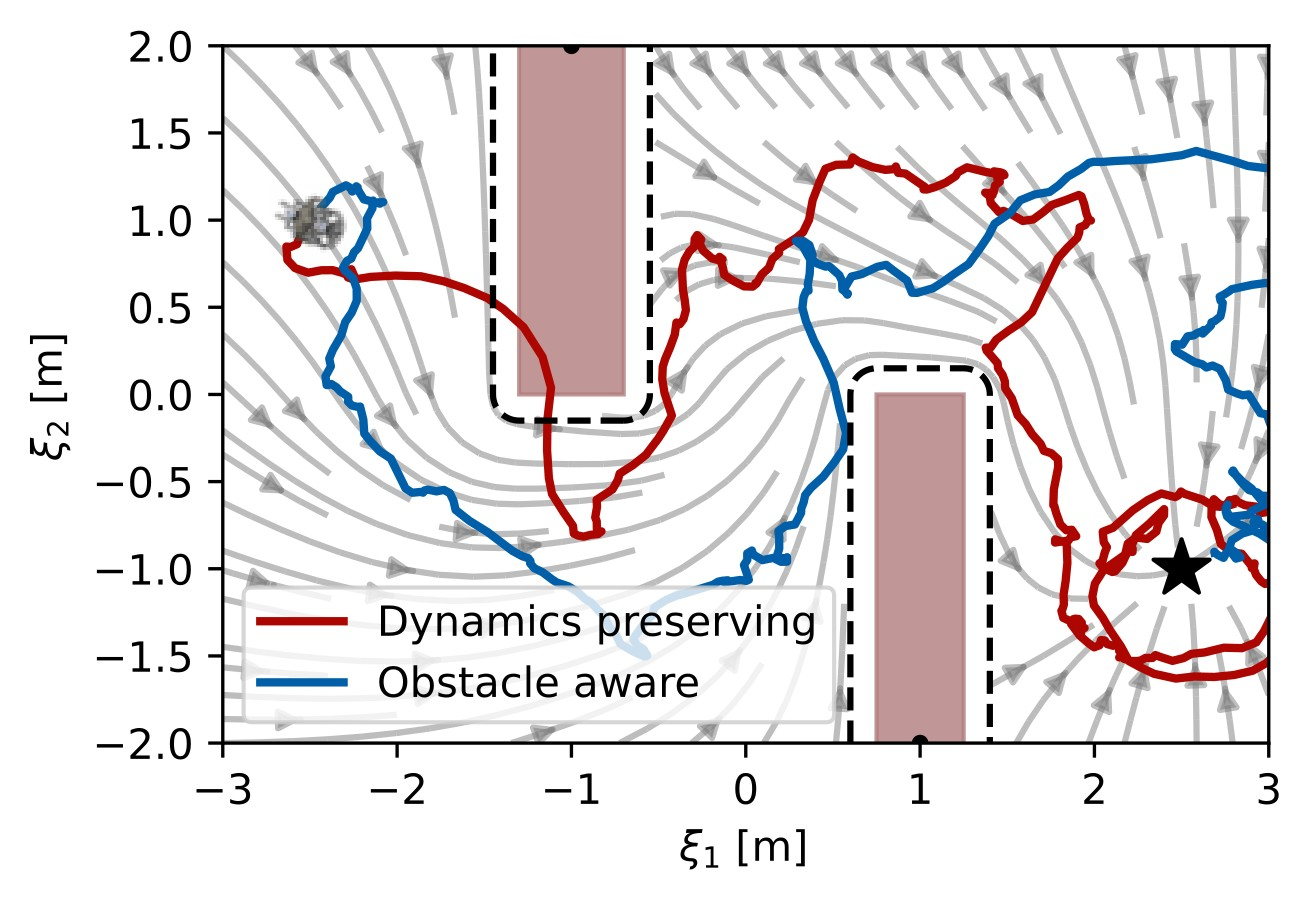
\includegraphics[width=\textwidth]{figures/trajectory_position_noise}}
      \caption{Trajectories with a standard deviation of the position-noise of 0.0 m.}
      \label{fig:trajectory_position_noise}
    \end{subfigure}
    \begin{subfigure}{\columnwidth}
    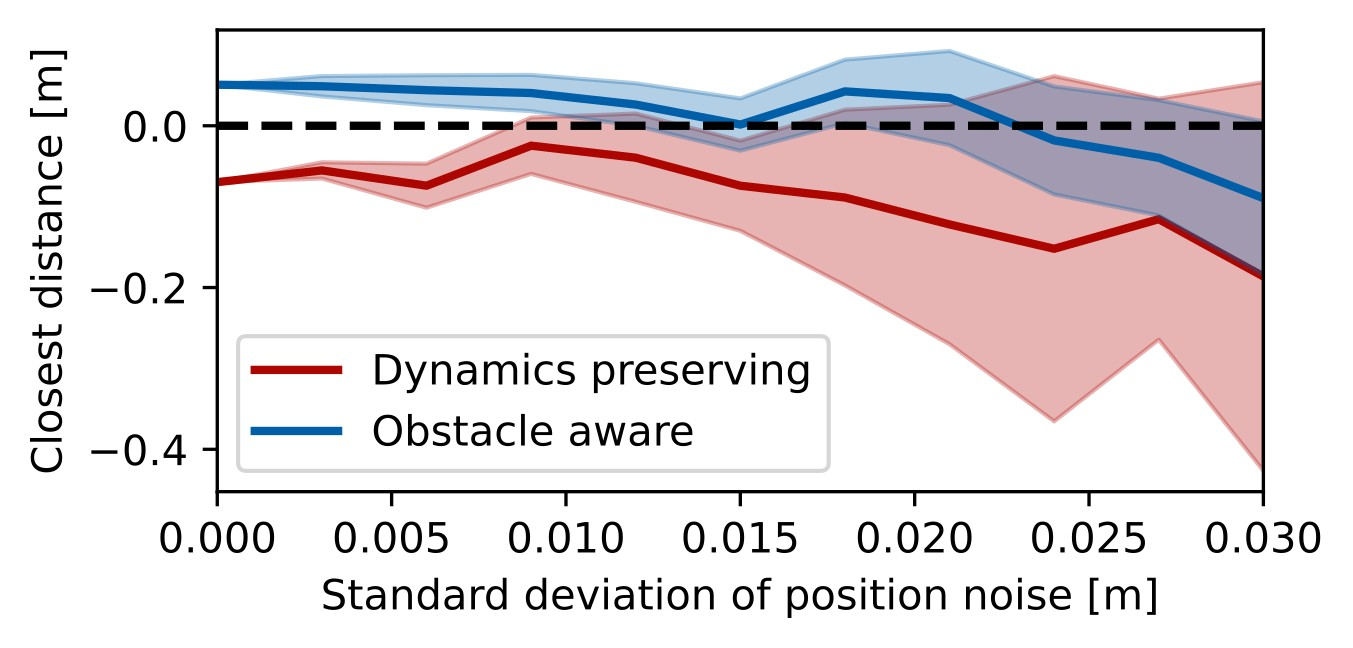
\includegraphics[width=\textwidth]{figures/comparison_position_noise}
      \caption{Closest distances concerning different noise levels over 10 epochs.}
      \label{fig:comparison_position_noise}
    \end{subfigure}
	\caption{The agent is navigating towards the attractor (black star) between two concave obstacles (a), while white noise acting on the agent's position. The velocity noise has a mean of zero, different variances between \qty{0.0}{m} and \qty{0.03}{m} are evaluated.}
\label{fig:position_noise}
\end{figure}


\subsubsection{Obstacle Aware Passivity Using a Robot Arm}
The controller was used to guide a 7 degree of freedom robot arm (Pand from Franka Emika) while avoiding collisions. The state $\vect \xi$ of the robot is the end effectors positions, and the obtained control acceleration.final 

The joint torque is obtained using inverse kinemtatics:
\begin{equation}
	\vecs \tau_q = \matr J^{\dag}(\vect q) 
	\begin{bmatrix} \matd D(\vecs \xi) \left( \vect f(\vecs \xi) - \dot{\vecs \xi} \right) \\  p^\alpha (\vecs \alpha - \vecs \alpha^a) \end{bmatrix}
	% \;\; \text{with} \;\;
	% \matr J^{\dag} = \matr J^T (\matr J \matr J^T)^{-1}
\end{equation}
using the Moore-Penrose pseudo inverse of the Jacobian $\matr J^{\dag} = \matr J^T (\matr J \matr J^T)^{-1}$. The angle $\vecs \alpha$ describes the end effector orientation, and the desired orientation is pointing downward with a quaternio value of $\vecs \alpha^a = [0, 1, 0, 0]$. For the substraction, we use quaternion representation to avoid singularities, but for the evaluation of the torque from the angular offset angle-axis represtation of the orientation is used.

The angular damping is chosesn as $p^\alpha = 5.5$.
The damping values are set as
$s^{\mathrm{obs}}=\, $ \qty{160}{s^{-1}},
$s^{\mathrm{DS}}= \,$ \qty{64}{s^{-1]}}, and
$s^{\mathrm{c}}= \,$ \qty{16}{s^{-1}}.
% multiplier = 8.0  # increase for faster but less stable
% self.linear_principle_damping = 8 * multiplier  # 50.
% self.linear_obstacle_damping = 20 * multiplier  # 60.
% self.linear_orthogonal_damping = 2 * multiplier  # 20.


The robot was set to move from initial position approximately at $\vecs \xi_0 = [0.3\mathrm{m}, 0.4\mathrm{m}, 0.3\mathrm{m},]^T$ to the attractor $\vecs \xi^a = [0.26 \mathrm{m}, -0.53\mathrm{m}, 0.33\mathrm{m}]^T$.
The motion is guided by dynamical system in the presence of a single squared box with axes length \qty{0.16}{m}, and a margin of \qty{0.12}{m}. The box is placed approximately at the center of start and attractior, but the precise loaction  is obtained at each time step using marke based vision system (optitrack). 
While passing the box, the robot is disturbed by a strong push $\vecs t_e$ towards the box. The sequence is repeated 10 times for both controllers, as well as for the undisturbed motion.

From the experimental results in Figure~\ref{fig:evaluation_on_robot_arm}, it is observed that using the obstacle ware controller, the robot is able stay on average \qty{0.15}{m} away from the obstacle surface. While for the dynamics preserving controller, the mean distance is below \qty{0.05}{m}, and many trajectories collide with the box. 
This results from a much weaker control force of the obstacle aware controller. Which has a high peak as soon as the disturbance occurs, at around \qty{1.45}{s}. Conversely, for the dynamics preserving trajecotry no such high peak occurs, and the controller only acts when the robot is almost in collision. In fact, the obstacle aware controller already show high forces before the disturbance, this additionally results in improved tracking of the avoidance trajectory as we've seen in Section~\ref{sec:position_noise}.


\begin{figure}
    \centering
   \begin{subfigure}{\columnwidth}
    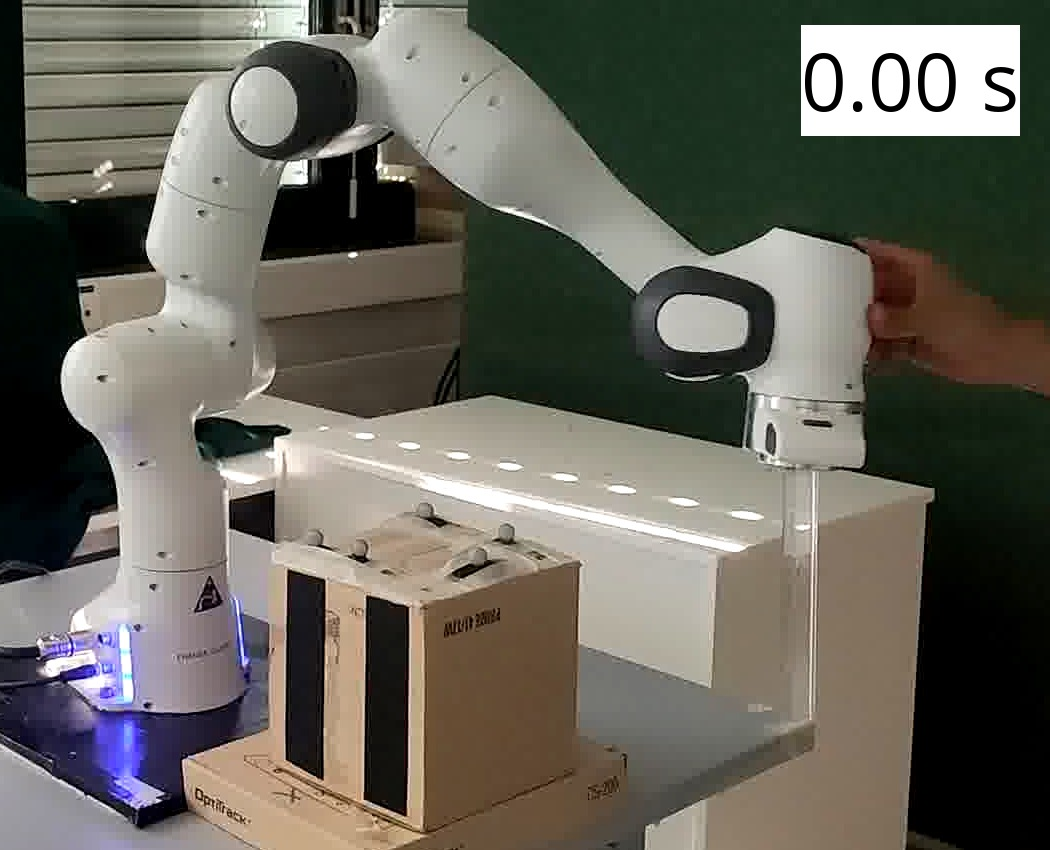
\includegraphics[width=0.49\textwidth]{figures/franka_sequence/franka_obstacle_aware016}\hfill%
    % 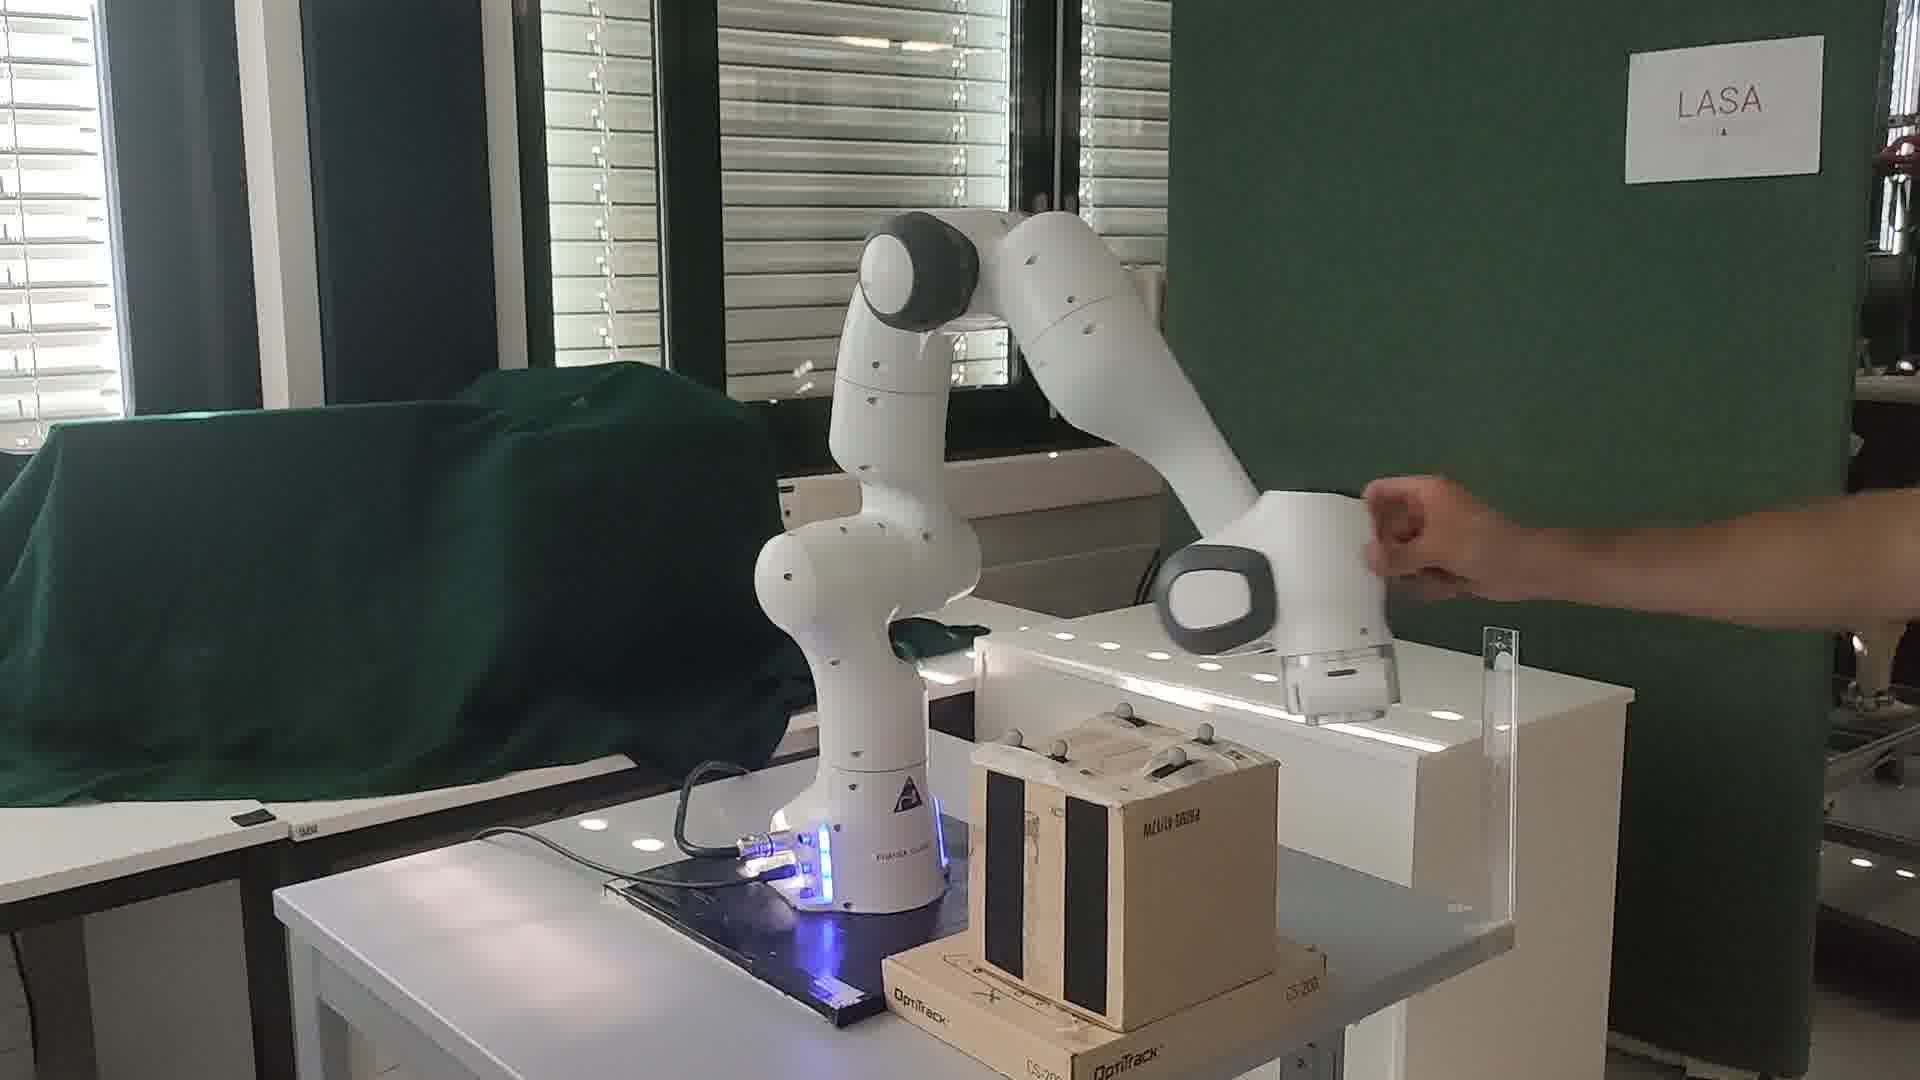
\includegraphics[width=0.33\textwidth]{figures/franka_sequence/franka_obstacle_aware018}\hfill%
    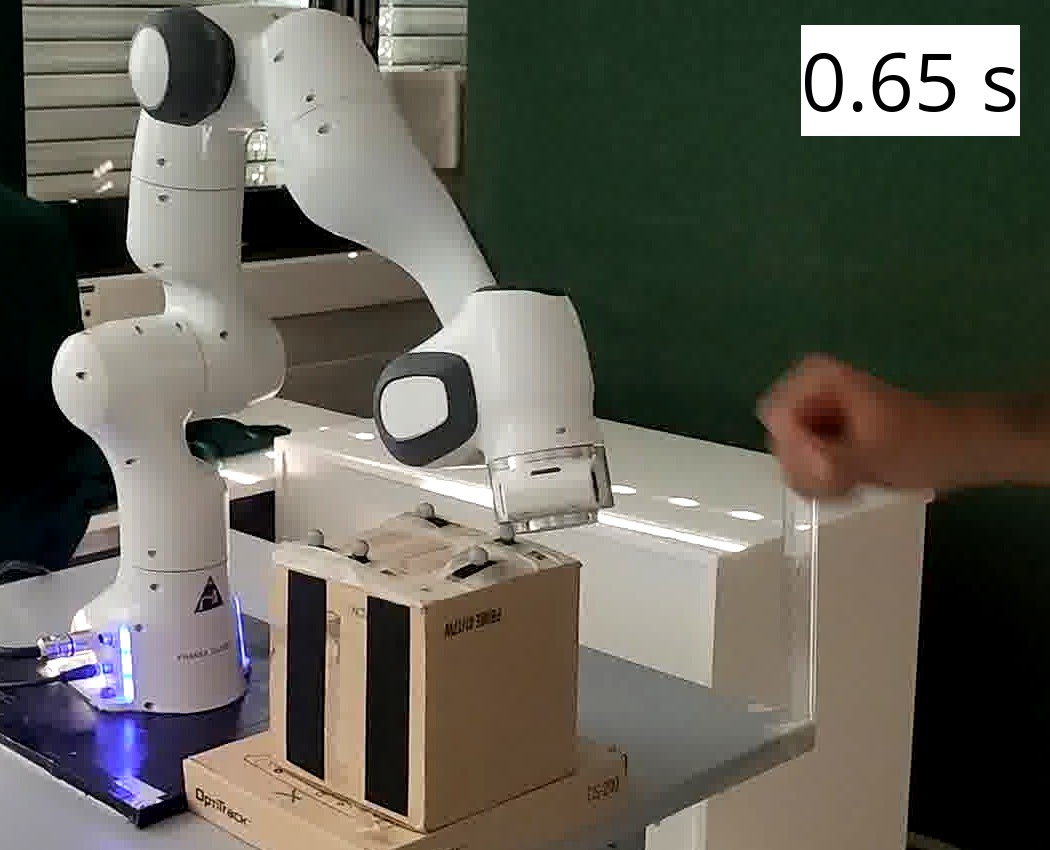
\includegraphics[width=0.49\textwidth]{figures/franka_sequence/franka_obstacle_aware020}
      \caption{Obstacle aware controller rejects repulsion and avoids collision}
      \label{fig:franka_sequence_obstacle_aware}
    \end{subfigure}
	\begin{subfigure}{\columnwidth}
    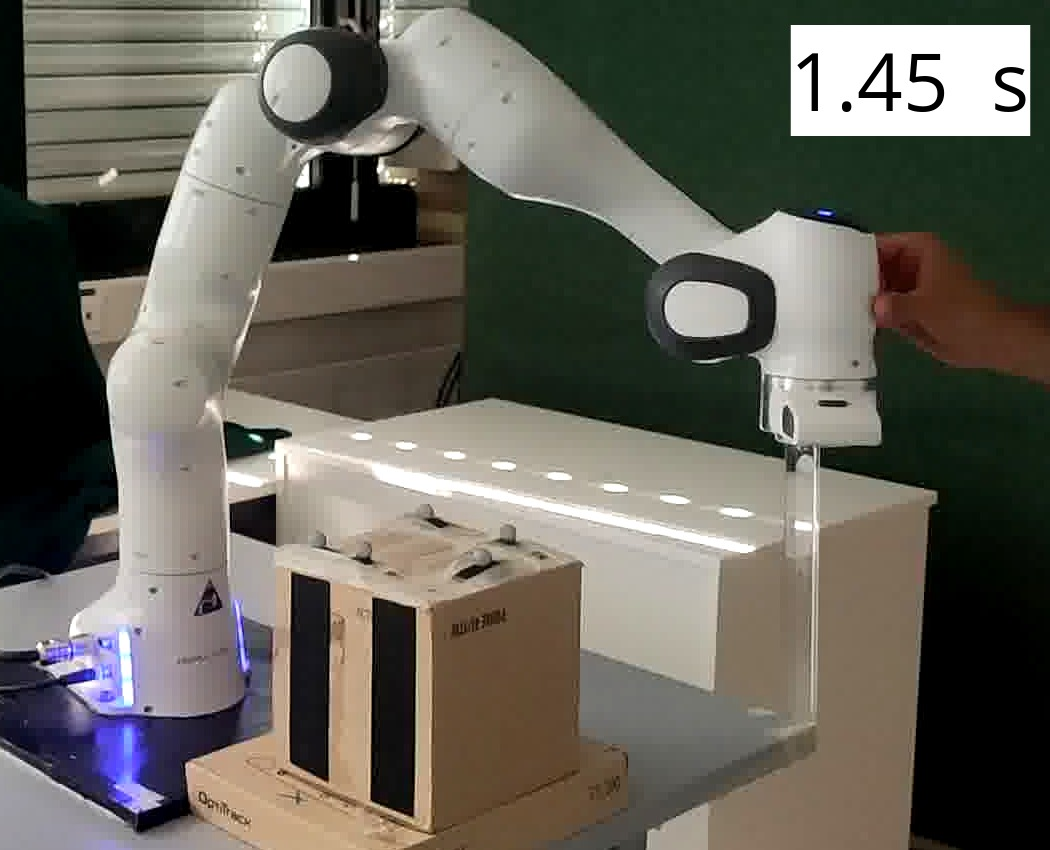
\includegraphics[width=0.49\textwidth]{figures/franka_sequence/franka_velocity_conserving021}\hfill%
    % 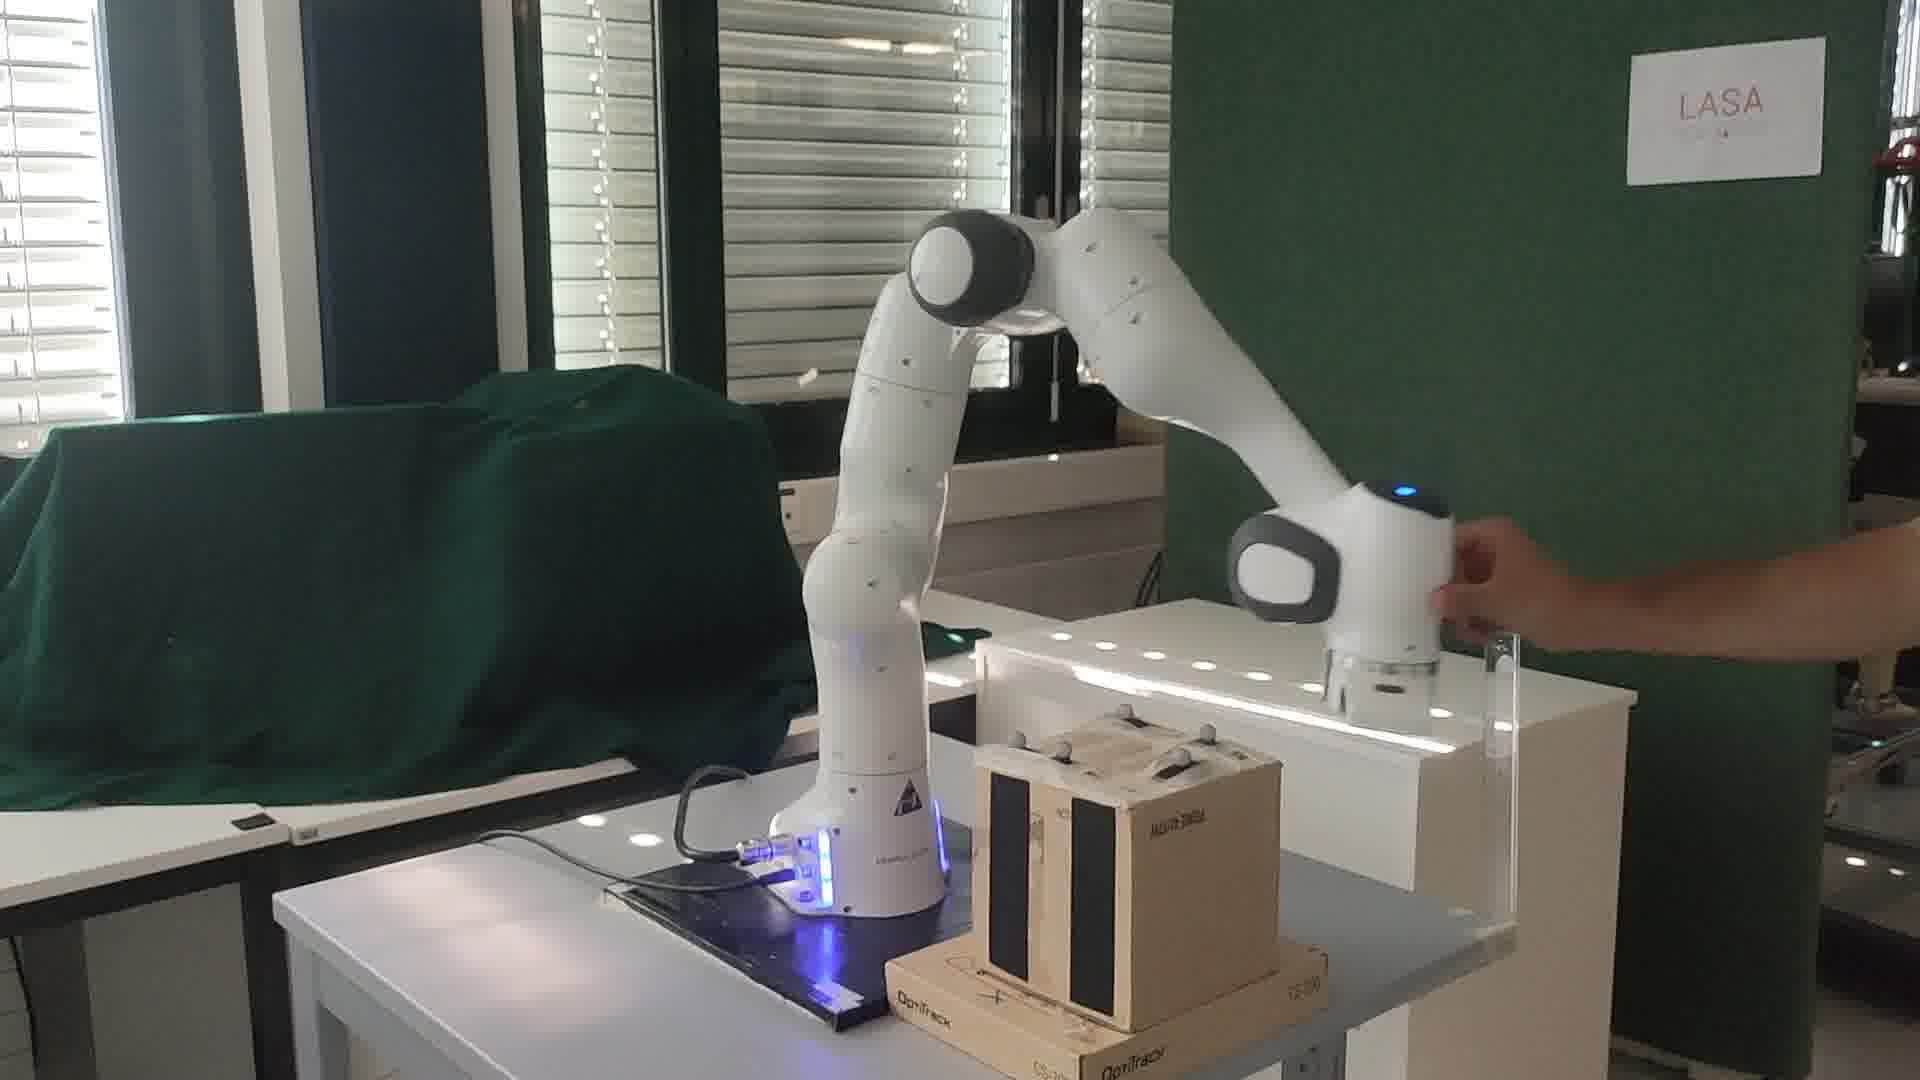
\includegraphics[width=-1.33\textwidth]{figures/franka_sequence/franka_velocity_conserving023}\hfill%
    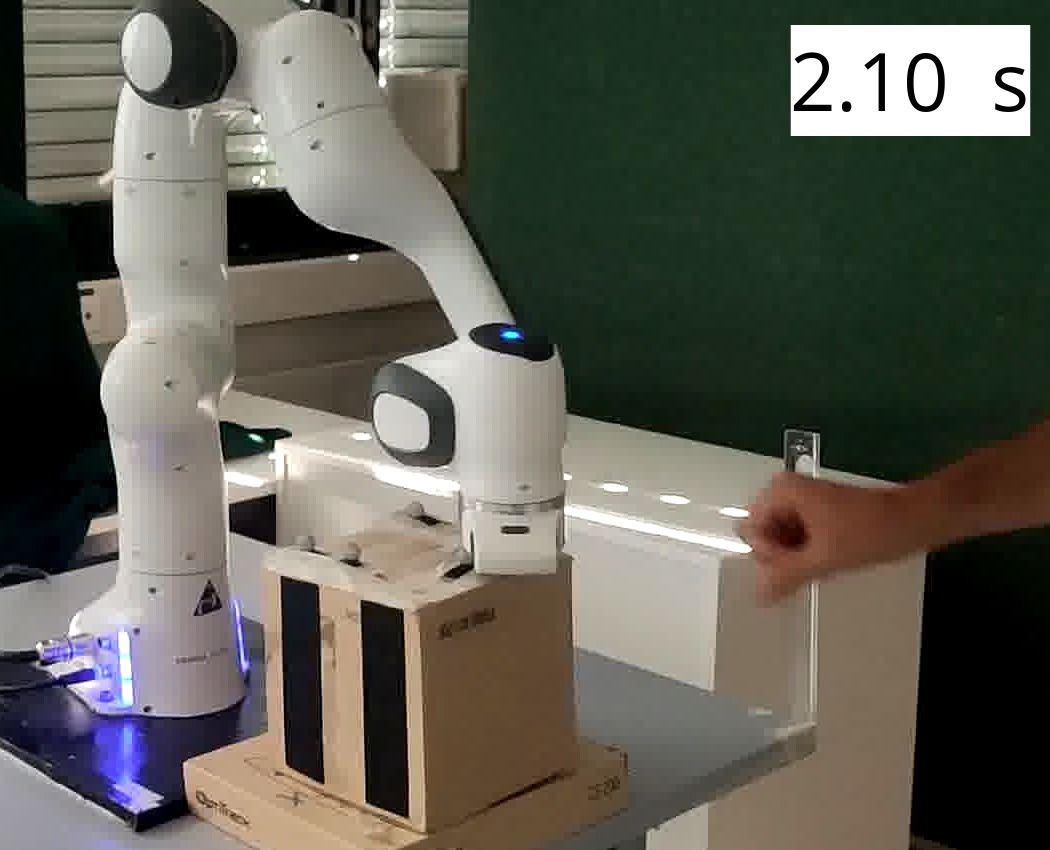
\includegraphics[width=0.49\textwidth]{figures/franka_sequence/franka_velocity_conserving025}\hfill%
      \caption{Dynamics preserving controller leads to collsion with obstacle}
      \label{fig:franka_sequence_obstacle_aware}
    \end{subfigure}
%    \caption{Comparison of the two control methods}
%    \label{fig:evaluation_on_robot_arm}
% \end{figure}
% \begin{figure}
%     \centering
    \begin{subfigure}{\columnwidth}
      \centerline{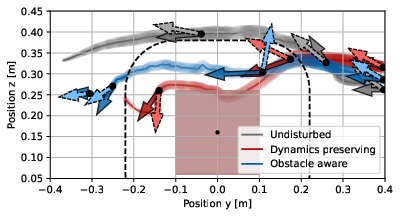
\includegraphics[width=\textwidth]{figures/robot_arm_trajectory_xyz}}
      \caption{The two control methods compared with the undisturbed trajectory. Wider line indicates higher x-value. The darker arrow is the actual, and the brighter the desired velocity.}
      \label{fig:robot_arm_trajectory_xyz}
    \end{subfigure}
    \begin{subfigure}{\columnwidth}
		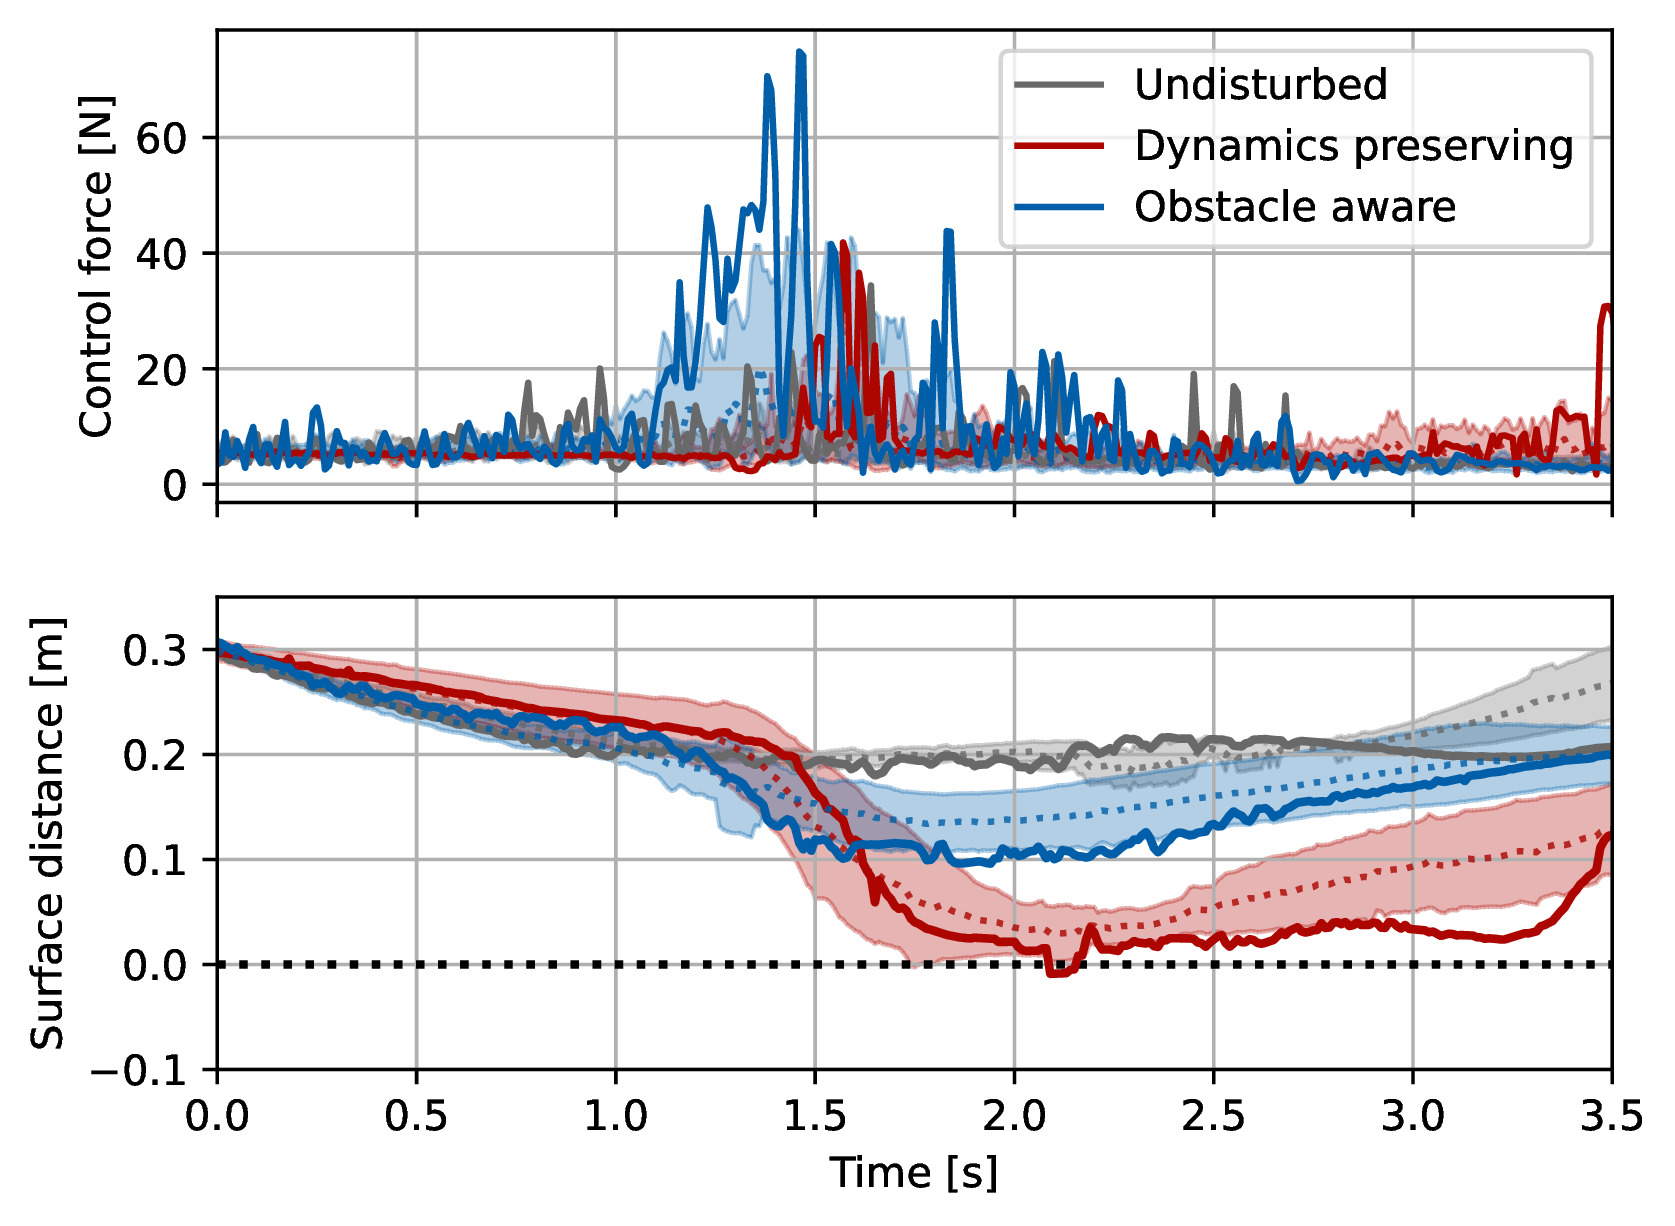
\includegraphics[width=\textwidth]{figures/trajectory_comparison_force_and_distance}
      \caption{The specific trajectory (full line), as well as average (dashed line) and variance (shaded area) over 10 runs are visualized. For the control force, mean and variance are evaluated in the logarithmic space.}
      \label{fig:trajectory_comparison_force_and_distance}
    \end{subfigure}
	\caption{Using the obstacle-aware passive controller, combined with a margin of 0.16m around the obstacle, the roboto arm is succesfully able to avoid the disturbance towards the obstacle. A similar disturbance has been applied to the robot arm over the 10 experimental runs. }  
    \label{fig:evaluation_on_robot_arm}
\end{figure}

\section{Discussion}
Overall, the simulated robot shows pleasing results. It has good tracking performances, compliance in the direction perpendicular to the motion, and great damping of the disturbances towards obstacles.
Away from obstacles, the controller presented shows similar behavior as the one in \cite{kronander2015passive}. When approaching one obstacle, the control gets damped more to avoid collisions without losing its tracking properties. This makes the proposed controller a suitable option to cumulate good tracking and safety regarding obstacle penetration.

\subsection{Applicability Approach}
Note, that the theoretical analysis from Theorem~\ref{theorem:passivity}, indicates passivity for any velocity-bounded, uniquely damped system. As a result, work such as the damping-based controller in  \cite{kronander2015passive} does not require an energy tank anymore.
Conversely, if the impedance controller has a proportional $\mathcal{K}$, the adaptive proportional term might induce instabilities even for stable desired dynamics as pointed out in \cite{ferraguti2013tank, kronander2016stability}.
